\documentclass[11pt,a4paper]{article}
\usepackage[T1]{fontenc}
\usepackage{lmodern}
\usepackage[margin=2.2cm]{geometry}
\usepackage{amsmath,amssymb}
\usepackage{graphicx}
\usepackage{booktabs}
\usepackage[font=small,labelfont=bf,skip=4pt]{caption}
\usepackage{xcolor}
\usepackage{microtype}
\usepackage{titlesec}
\usepackage[colorlinks=true,linkcolor=black,citecolor=black,urlcolor=blue!50!black]{hyperref}

\graphicspath{{../../outputs/paper_figures/}{../outputs/paper_figures/}}
\titleformat{\section}{\large\bfseries}{\thesection}{0.6em}{}
\titleformat{\subsection}{\normalsize\bfseries}{\thesubsection}{0.6em}{}
\titlespacing*{\section}{0pt}{10pt}{4pt}
\titlespacing*{\subsection}{0pt}{7pt}{3pt}
\setlength{\parskip}{3pt}
\setlength{\textfloatsep}{8pt}
\setlength{\floatsep}{6pt}
\setlength{\intextsep}{6pt}

\newcommand{\Qstar}{Q2$^{*}$}

\begin{document}

\begin{center}
{\LARGE\bfseries Fast and Fair: Scheduling and Rebalancing\\[2pt] a Heterogeneous GPU Cluster}\\[6pt]
{\large 2026 MCM Senior Group --- Problem B}
\end{center}

\section*{Summary}

We study a three-month trace of 224,112 jobs submitted to 4,278 GPU servers carrying 10,412 GPUs of six models. GPU work is concentrated in a few long jobs: jobs longer than seven days are 6.0\% of submissions but carry 77.0\% of the work. Demand is also badly matched to supply. The A10 pool holds 24.0\% of the GPUs, yet its jobs request 2.06 times its 90-day capacity, while every other pool requests between 0.58 and 1.16 times its own.

We formulate placement as a node-level feasibility condition and evaluate queue policies with an exact discrete-event simulator that runs every job to completion. Because the A10 pool is saturated, queue order decides who waits rather than how much work is done. Shortest-job-first cuts the mean wait from 447\,h under first-come-first-served to 16.6\,h but leaves months-long jobs waiting up to 3,017\,h. Our logarithmic aging rule, which ranks jobs by $\ln d_j + a_j/T$, keeps the mean at 31.2\,h with $T=7$ days and brings the maximum down to 1,515\,h, close to the first-come-first-served level.

Queue order cannot create A10 capacity, but idle GPUs on other models can supply it. In our routing mechanism, A100 and H800 pools whose own queues are empty pull eligible A10 jobs, subject to runtime limits of 75 days on A100 and 30 days on H800. On ten held-out samples of eligible jobs, this lowers the cluster mean wait to 3.6\,h and the time to finish all jobs from 247 to 211 days, while native donor users wait at most 0.22\,h longer on average, even when migrated jobs run 20\% slower. A protected variant guarantees that no A10 job is delayed by routing, at a mean wait of 10.5\,h.

\noindent\textbf{Keywords:} gang scheduling; discrete-event simulation; aging; heterogeneous clusters; rebalancing

\section{Introduction and Assumptions}

A GPU cluster must decide which waiting job starts next, where its workers run, and, when some GPU models are scarce while others sit idle, whether work may move between models. The three questions of Problem B follow this order, and so does our paper. We start from the data (Section~2), because the shape of the workload determines what a good scheduler must achieve. The analysis yields two facts that drive the rest of the paper. Long jobs dominate the work, which shapes the queue policy of Section~3. The A10 pool is overloaded, which motivates the cross-model routing of Section~4, since no queue policy can clear a backlog caused by missing capacity.

Our approach builds on well-established scheduling ideas and adapts them to the structure of this trace. First-come-first-served with backfilling is the default in high-performance computing~\cite{lifka,slurm}, and shortest-job-first is the classical way to minimize mean waiting time. Aging, which raises the priority of jobs that have waited long, is the classical remedy for the starvation that shortest-first rules cause. The trace itself comes from a production GPU cluster~\cite{ali}, and it differs from textbook settings in two ways. Runtimes span six orders of magnitude, and one GPU model is persistently short of capacity. Both features turn out to require modifications of the classical rules. Figure~\ref{fig:overview} previews the resulting system: every pool orders its queue by logarithmic aging and places workers node by node, and idle A100 and H800 pools pull eligible A10 jobs under runtime limits. Throughout, we evaluate rules by replaying the full trace in a simulator that executes them exactly as an online scheduler would, and we compare them by the waiting time they impose on each class of users.

\begin{figure}[ht]
\centering
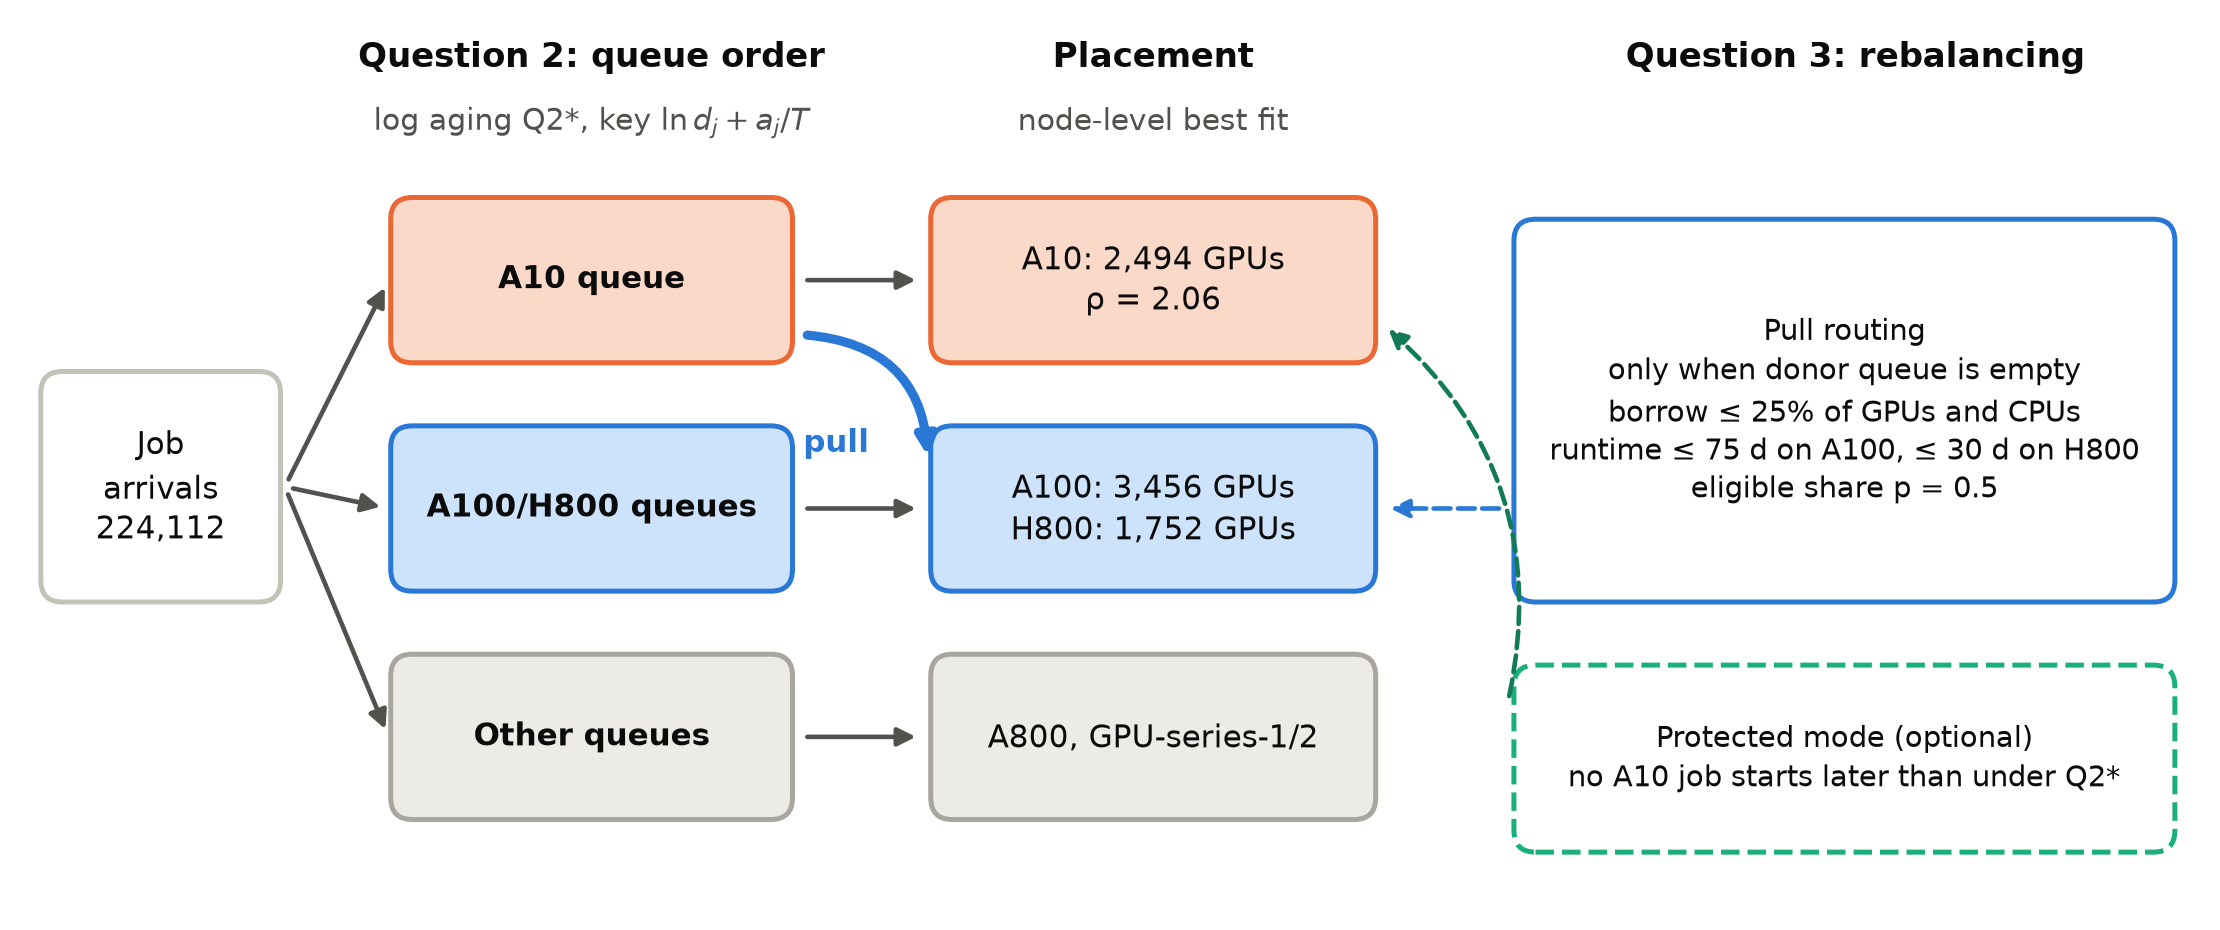
\includegraphics[width=0.9\textwidth]{fig_overview.png}
\caption{Overview of the proposed system. Each pool orders its queue by logarithmic aging (Section~3) and places workers by node-level best fit; idle A100 and H800 pools pull eligible A10 jobs under pool-specific runtime limits (Section~4), optionally with a protected mode that guarantees no A10 job starts later.}\label{fig:overview}
\end{figure}

Job $j$ requests GPU model $k(j)$ and consists of $m_j$ identical workers, each needing $g_j$ GPUs and $c_j$ vCPUs. It arrives at time $a_j$, starts at $s_j$, runs for $d_j$, and waits $w_j=s_j-a_j$; its GPU work is $W_j=g_jm_jd_j$. Node $n$ has model $k(n)$, $G_n$ GPUs and $C_n$ vCPUs.

We adopt the constraints of the problem. All workers of a job start simultaneously, and each worker's GPUs and CPUs lie on one node of the requested model (A1). Jobs run without preemption for exactly $d_j$, which is known on arrival (A2). All nodes are idle at $t=0$, and the scheduler sees only jobs that have arrived (A3). We add three assumptions of our own. The trace is a closed workload (A4): every job is scheduled until it completes. Waiting times therefore include jobs that start after day 90, while throughput and allocation are measured over the 90-day window. Cutting the simulation at day 90 instead would silently drop the longest waits, exactly the quantity a fair policy must control. Substitution in Question~3 is limited (A5). A fixed share $p=0.5$ of A10 jobs, selected by a hash of the job identifier, may run on A100 or H800; they represent jobs whose code is compatible and whose owners accept substitution. Selecting by hash keeps eligibility independent of runtime and arrival time and makes every experiment reproducible; different hash seeds give different but equally plausible sets of eligible jobs, which we later use as independent samples. A migrated worker keeps its GPU and CPU request and runs at relative speed $v$, so its runtime becomes $d_j/v$. We study $v=1$ and the pessimistic $v=0.8$, and ignore migration overhead. Finally, donor protection is a management constraint (A6): for every donor model, the mean wait of native jobs may rise by at most 0.5\,h and their 95th-percentile wait by at most 2\,h, relative to the same schedule without routing. These bounds are deliberately tight. Donor users gain nothing from routing, so the operator should be able to promise them that sharing their GPUs costs at most a small, predictable delay.

\section{Question 1: Understanding the Workload}

The trace is clean. It has no missing values, duplicate identifiers or unknown models, and every job fits into its model's pool when the pool is empty. We keep the 73 fractional and one zero CPU request as given, and we keep every extreme job, because the extremes are where the work lies.

Requested work totals 24.6 million GPU-hours and is spread very unevenly. The median job runs 22 minutes, while the longest runs about 184 days. Jobs of at most one hour make up 70.8\% of submissions but carry only 0.7\% of GPU work, whereas jobs longer than seven days make up 6.0\% of submissions and carry 77.0\%. The top 1\% of jobs by work contribute 43.3\% of it (Figure~\ref{fig:workload}; Gini coefficient 0.95). These heavy jobs are mostly long rather than wide, since 73.9\% of all jobs use a single GPU. The H800 pool is the exception: 61.9\% of its jobs have several workers, the median job uses 16 GPUs, and one job requests 1,456 of the pool's 1,752 GPUs. This difference will matter when we decide which pools may lend capacity. CPUs, by contrast, are rarely the binding resource. A10 jobs request about 24 vCPU-hours per GPU-hour, while each A10 node offers 128 vCPUs for its single GPU, so in the A10 pool the GPU count alone decides whether a job fits.

\begin{figure}[ht]
\centering
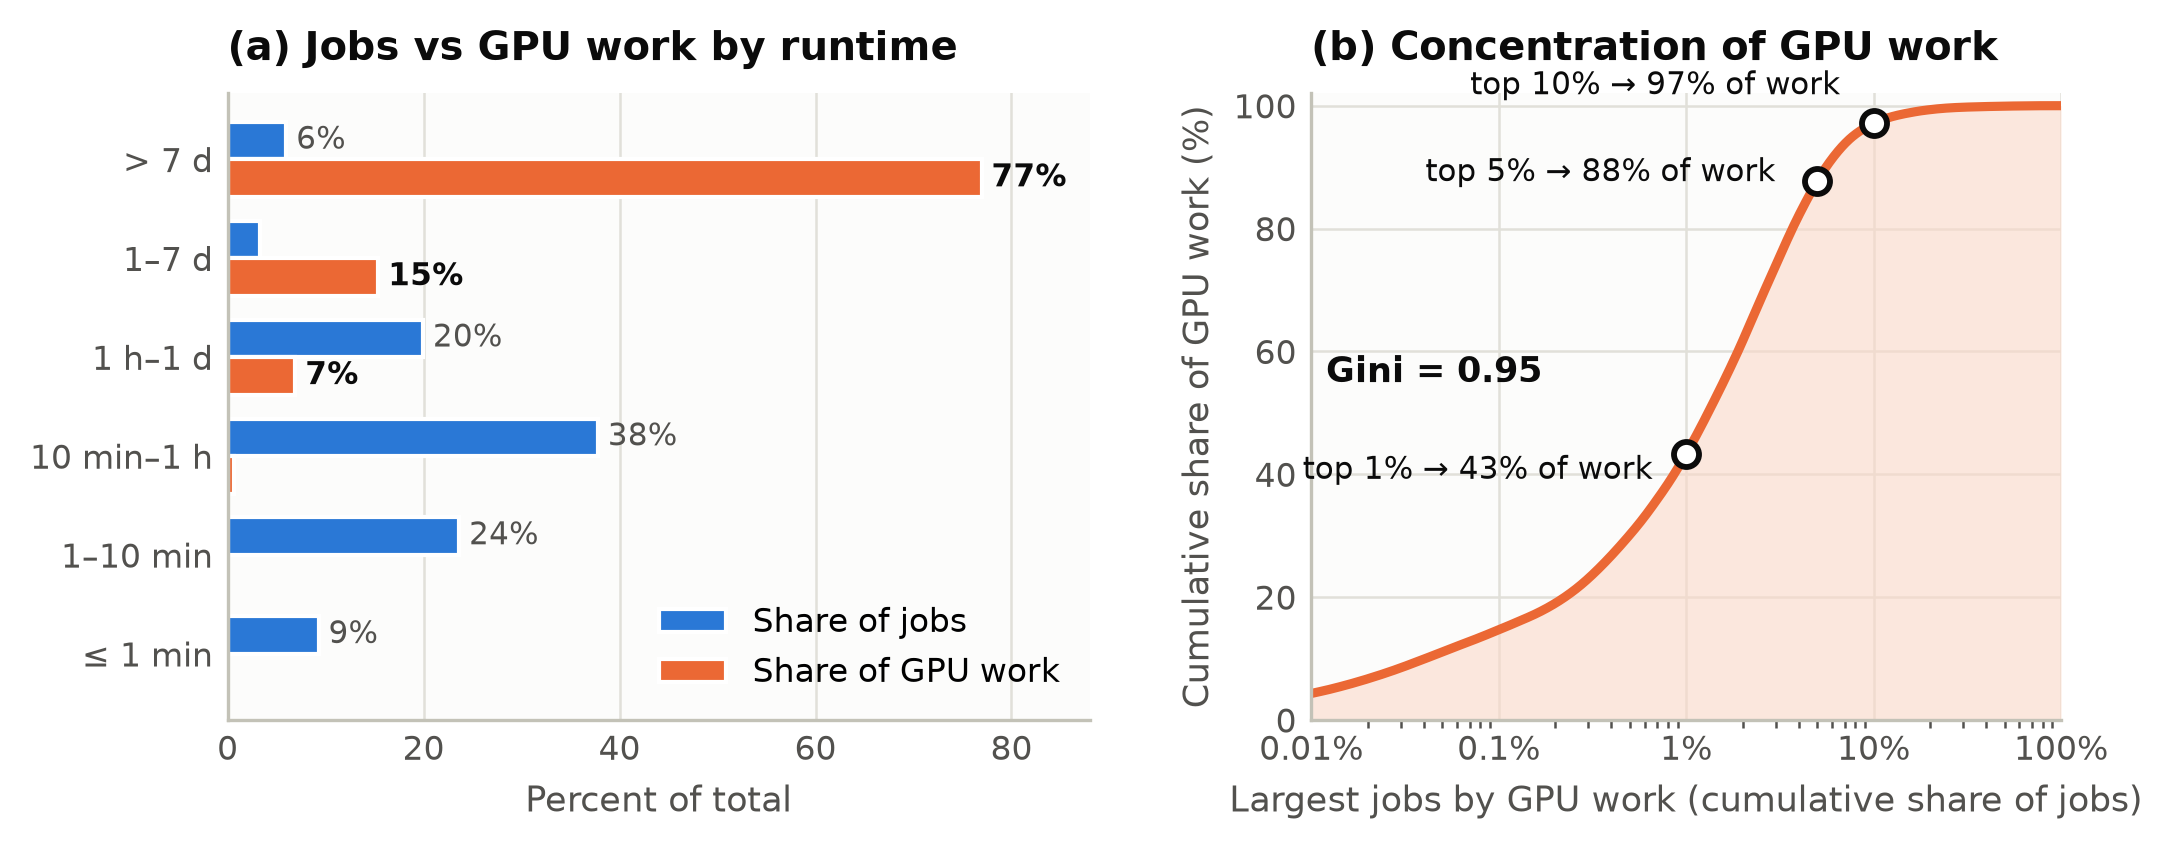
\includegraphics[width=0.97\textwidth]{fig1_workload.png}
\caption{(a) Share of jobs and of GPU work by runtime class. (b) Cumulative share of GPU work carried by the largest jobs.}\label{fig:workload}
\end{figure}

Concentration alone would not cause congestion if capacity matched demand. We compare the two through the workload-to-capacity ratio
\begin{equation}
\rho_k=\frac{\sum_{j:k(j)=k} W_j}{90\,\text{d}\cdot\sum_{n:k(n)=k} G_n},
\end{equation}
which compares the work submitted for model $k$ with what its GPUs can perform in 90 days. Table~\ref{tab:models} shows a stark mismatch. The A10 pool receives 45.2\% of all GPU work on 24.0\% of the GPUs, about twice what it can deliver, while A100, A800, H800 and GPU-series-2 receive well under their capacity.

\begin{table}[ht]
\centering\small
\caption{Demand and capacity by GPU model.}\label{tab:models}
\begin{tabular}{lrrrr}
\toprule
GPU model & GPUs & Jobs & Share of GPU work & $\rho_k$\\
\midrule
A10 & 2,494 & 111,284 & 45.2\% & \textbf{2.06}\\
A100-SXM4-80GB & 3,456 & 80,877 & 24.1\% & 0.80\\
GPU-series-1 & 1,558 & 9,643 & 15.8\% & 1.16\\
H800 & 1,752 & 4,716 & 9.0\% & 0.58\\
GPU-series-2 & 976 & 13,633 & 5.0\% & 0.58\\
A800-SXM4-80GB & 176 & 3,959 & 0.9\% & 0.61\\
\bottomrule
\end{tabular}
\end{table}

The ratio does not say when demand arrives, so we also compute the GPU demand that would exist if every job started on arrival (Figure~\ref{fig:supply}b). A10 demand stays above capacity for 99.6\% of the window and averages 1.45 times capacity, rising to about 1.6 times between days 50 and 65. Its pressure is therefore persistent rather than a passing burst that a few days of queueing could absorb. The other models fluctuate below their capacity throughout. GPU-series-1, despite $\rho_k>1$, never exceeds 0.95 of capacity at arrival; its high ratio comes from long jobs that run past day 90. In addition, 3,512 jobs carrying 23.1\% of all work arrive at $t=0$, so the cluster starts with a large backlog. With fixed capacity and strict model matching, the A10 work alone occupies the whole A10 pool for 185.8 days, which bounds from below the time needed to finish all jobs.

\begin{figure}[ht]
\centering
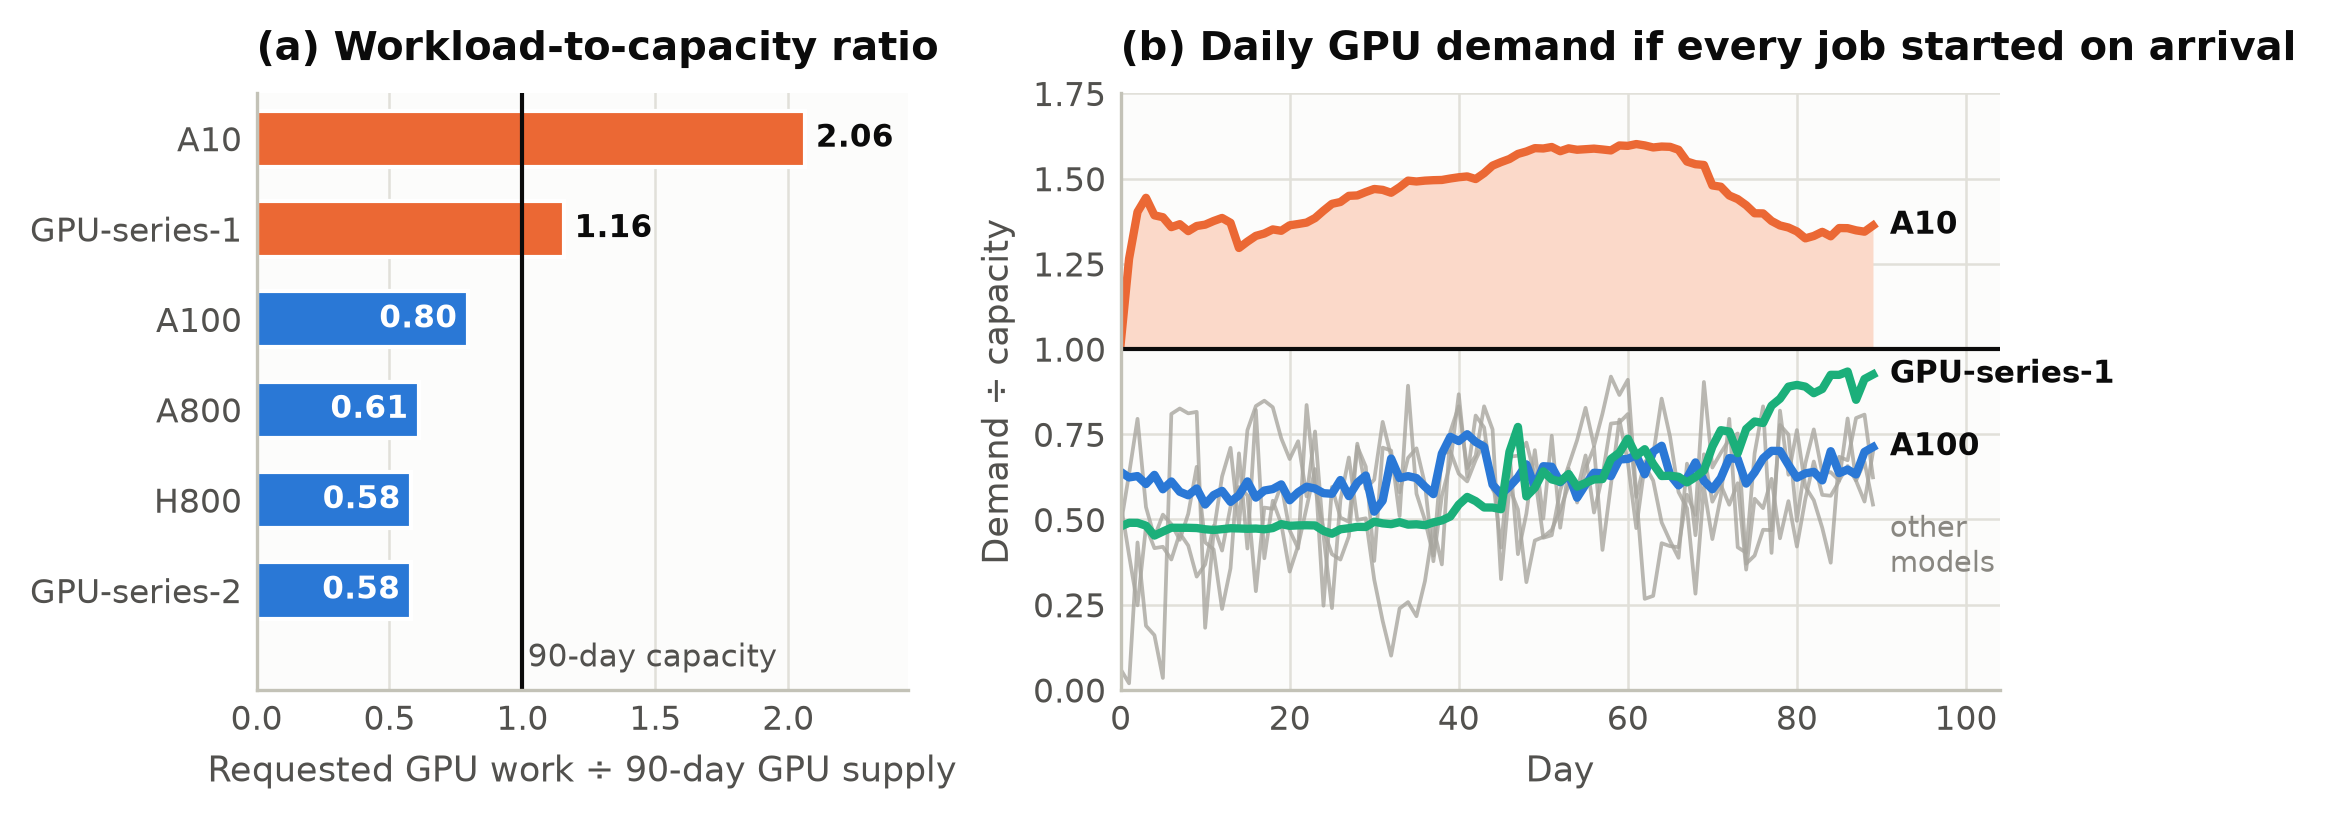
\includegraphics[width=0.97\textwidth]{fig2_supply_demand.png}
\caption{(a) Workload-to-capacity ratio by GPU model. (b) Daily GPU demand relative to capacity if every job started on arrival.}\label{fig:supply}
\end{figure}

These findings set the agenda. Because A10 is overloaded on capacity grounds, a queue policy can only decide which A10 jobs wait. Because long jobs carry the work while short jobs make up most users, a good policy must keep short jobs responsive without starving long ones, and must be judged beyond the mean. And because other models have spare GPUs exactly when A10 is congested, moving work across models is the natural remedy once the queue policy is settled.

\section{Question 2: Scheduling and Placement}

\subsection{Placement model and simulation}

Before choosing which job to start, we need to know whether a job can start. Let $\hat G_n$ and $\hat C_n$ be the GPUs and vCPUs currently free on node $n$. Node $n$ can host $q_{jn}=\min\big(\lfloor \hat G_n/g_j\rfloor,\ \lfloor \hat C_n/c_j\rfloor\big)$ workers of job $j$ (the CPU term is omitted when $c_j=0$). Because the workers of a job are identical, the job can start now if and only if
\begin{equation}
\textstyle\sum_{n:\,k(n)=k(j)} q_{jn}\ \ge\ m_j .
\end{equation}
Consider the example job of the problem statement, with four workers that each need 2 GPUs and 16 vCPUs. An idle 8-GPU A100 node with 128 vCPUs gives $q_{jn}=\min(4,8)=4$ and can host the whole job, whereas a node with only 3 free GPUs gives $q_{jn}=1$ and must be combined with others. When a job can start, we place its workers by best fit, filling first the feasible nodes with the fewest free worker slots so that whole nodes stay free for wide jobs. Scheduling then becomes a sequencing problem. Its offline version contains multidimensional bin packing and is NP-hard, and an online scheduler does not know future arrivals anyway, so we study online priority rules and evaluate them by simulation.

Our simulator advances from event to event. At each event time it releases every finishing job, admits every arriving job, and lets each affected pool start jobs according to its policy, continuing until the last job completes; a full replay takes 6--30 seconds. All ties are broken deterministically, and each scheduling decision costs a heap operation plus a scan over the nodes of one pool, so the scheduler itself is cheap enough for real-time use. An independent checker in exact decimal arithmetic rebuilds every node's occupancy from the output and confirms that capacities are never exceeded, that all workers of a job start together, that no job starts before it arrives, and that all runtimes are correct.

We judge a schedule by several complementary measures, because each answers a different question. The mean wait measures the responsiveness experienced by a typical job. The 99th-percentile and maximum waits expose starvation, which the mean hides when most jobs are short. The number of jobs finished by day 90 and the day on which the last job finishes describe how quickly the backlog clears. The share of GPU capacity allocated within the window shows whether a policy wastes resources. Breaking the mean wait down by runtime class shows which users pay for an improvement. No single measure captures all of these concerns, so we state explicitly which ones each choice trades against the others.

\subsection{Queue policies}

All policies share the placement rule and differ only in the order in which they serve the queue. A pool starts its head-of-queue job whenever it fits and otherwise waits, so the order fully determines who goes next. This strict head blocking leaves some GPUs briefly idle, but it guarantees that a wide job at the head cannot be overtaken indefinitely by narrow jobs that happen to fit, and it makes the policies directly comparable. First-come-first-served (FCFS) orders by arrival time and shortest-job-first (SJF) by runtime. Backfilling refines FCFS by computing the earliest start $t^*$ of the head job and letting a later job start now if it fits and finishes by $t^*$.

FCFS ignores that most users submit short jobs, and SJF ignores how long a job has waited. Aging combines the two by giving each waiting job a score that falls as it waits and serving the smallest score first. We study a linear form $s_j(t)=d_j-\alpha(t-a_j)$ and a logarithmic form $s_j(t)=\ln d_j-(t-a_j)/T$. In both, the term in $t$ is common to all waiting jobs, so ranking by $s_j(t)$ is equivalent to ranking by the fixed keys $d_j+\alpha a_j$ and $\ln d_j+a_j/T$, and one priority heap implements either rule. The two forms trade runtime against waiting differently. Under the linear form a job must wait $(d_L-d_S)/\alpha$ longer to outrank one that is shorter by $d_L-d_S$; under the logarithmic form, a job that arrived $T\ln(d_L/d_S)$ earlier outranks one that is $d_L/d_S$ times shorter. With $T=7$ days, for example, a 100-day job outranks newly arriving one-hour jobs after about 54 extra days ($7\ln 2400$). Since runtimes span six orders of magnitude, only a ratio-based rule treats short and long jobs on the same footing.

\subsection{Results and choice of policy}

First, what the policies cannot change. Under FCFS the A10 pool is 99.9\% allocated over 90 days and, while its queue is non-empty, idles for only 1,530 GPU-hours. Backfilling, which exists to fill idle resources, therefore improves the mean wait by only 0.3\%, and FCFS and SJF allocate almost the same share of the cluster (69.5\% and 69.4\%). The policies differ in who waits, not in how much work is done.

\begin{table}[ht]
\centering\small
\caption{Queue policies without routing.}\label{tab:policies}
\begin{tabular}{lrrrrr}
\toprule
Policy & Mean wait & P99 wait & Max wait & Done by & Last completion\\
 & (h) & (h) & (h) & day 90 & (day)\\
\midrule
FCFS & 447.3 & 1,416 & 1,423 & 164,886 & 243.3\\
SJF & 16.6 & 366 & 3,017 & 217,494 & 309.7\\
Linear aging, $\alpha=1$ & 18.4 & 707 & 2,842 & 217,192 & 302.4\\
\textbf{Log aging, $T=7$ d (\Qstar)} & \textbf{31.2} & 1,098 & \textbf{1,515} & 215,229 & \textbf{247.1}\\
Linear aging, $\alpha=100$ & 432.9 & 1,394 & 1,421 & 165,868 & 243.2\\
\bottomrule
\end{tabular}
\end{table}

Within this fixed amount of work, SJF achieves the lowest mean wait (Table~\ref{tab:policies}), and its benefit is broad: it lowers the mean wait of every runtime class relative to FCFS (Figure~\ref{fig:queue}b), from 503\,h to 0.03\,h for jobs under one hour and even from 481\,h to 270\,h for jobs over seven days. Its cost falls on a narrow tail. Only 1.1\% of jobs wait longer than under FCFS, but those wait 770\,h longer on average, and all 1,525 jobs that wait more than 1,000\,h are A10 jobs running 50--184 days. The tail sits in the A10 pool for a simple reason. In pools with spare capacity a long job eventually finds free GPUs, but in the overloaded A10 pool new short jobs arrive faster than they can be served and always rank ahead, so a months-long job waits until the arrivals thin out near the end of the trace. Because these jobs start late, the last job finishes on day 310 instead of day 243.

Aging is meant to close this gap, and Figure~\ref{fig:queue}a shows that its form decides whether it does. Linear aging jumps almost directly from SJF to FCFS: it behaves like SJF for $\alpha\le0.3$, while for $\alpha\ge3$ the mean wait already exceeds 180\,h, because a 100-day job needs $100/\alpha$ extra days to pass new short jobs. Logarithmic aging traces a much better curve. At $T=7$ days it halves SJF's maximum wait and brings the last completion within four days of FCFS, while the mean stays in the tens of hours.

\begin{figure}[ht]
\centering
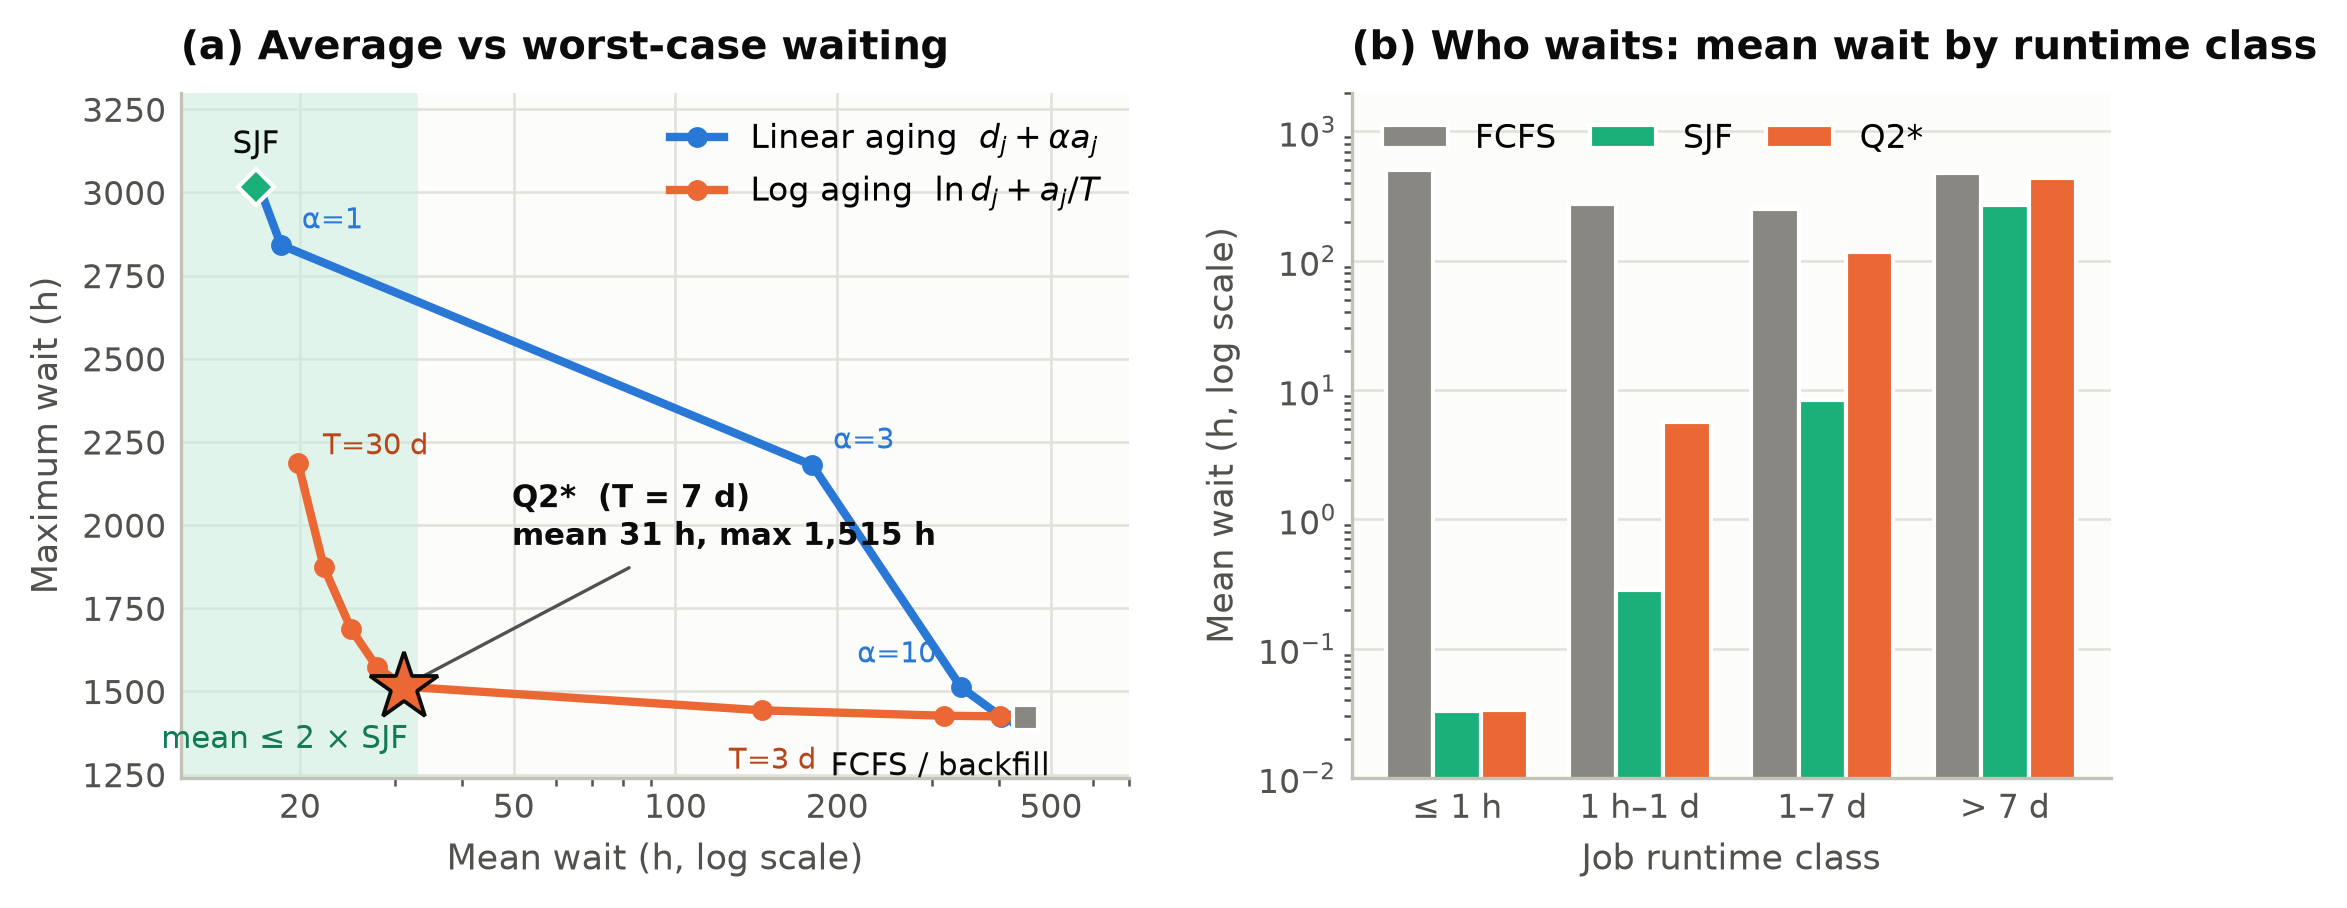
\includegraphics[width=0.97\textwidth]{fig3_queue_policies.png}
\caption{(a) Mean versus maximum wait for linear and logarithmic aging; the shaded band satisfies requirement C2. (b) Mean wait by runtime class under FCFS, SJF and \Qstar.}\label{fig:queue}
\end{figure}

To choose a policy we impose two requirements. C1: no runtime class may have a higher mean wait than under FCFS, so no group is worse off than under the simplest fair rule. C2: the overall mean wait may be at most twice that of SJF. Of the 22 policies tested (FCFS, SJF, two backfilling variants, 12 linear and 6 logarithmic aging settings), 11 satisfy both, and among them logarithmic aging with $T=7$ days has the smallest maximum wait. The price is a wider spread of moderate delays: the 99th-percentile wait rises from 366\,h under SJF to 1,098\,h, while the number of jobs waiting longer than FCFS's maximum falls from 1,199 to 159. A tighter budget of 1.5 times the SJF mean would select $T=30$ days (19.8\,h mean, 2,188\,h maximum), so $T$ acts as the operator's dial between average responsiveness and the worst case.

We adopt this policy, denoted \Qstar, in every pool. \Qstar\ settles how waiting is shared within each pool but leaves the A10 backlog untouched: A10 jobs still wait 62.4\,h on average while other pools have capacity to spare. This is the problem of Question~3, and \Qstar\ serves as its baseline.

\section{Question 3: Rebalancing Across GPU Models}

\subsection{Measuring the imbalance and pull routing}

Let $I_m(t)$ be the idle GPUs of pool $m$ and $Q_{A10}(t)$ the GPUs requested by waiting A10 jobs. For the donor set $\mathcal D=\{\text{A100, A800, H800, GPU-series-2}\}$, the stranded capacity
\begin{equation}
I_{\text{strand}}=\int_0^{90\,\text{d}}\min\Big(\textstyle\sum_{m\in\mathcal D} I_m(t),\ Q_{A10}(t)\Big)\,dt
\end{equation}
is the GPU time that sat idle on other models while A10 jobs waited. Under \Qstar\ it amounts to 3.68 million GPU-hours, about two-thirds of the A10 pool's 90-day capacity. Figure~\ref{fig:stranded}a shows how it builds up: from day 40 onward, waiting A10 demand climbs past 4,000 GPUs while 2,000 to 3,000 donor GPUs stand idle.

\begin{figure}[ht]
\centering
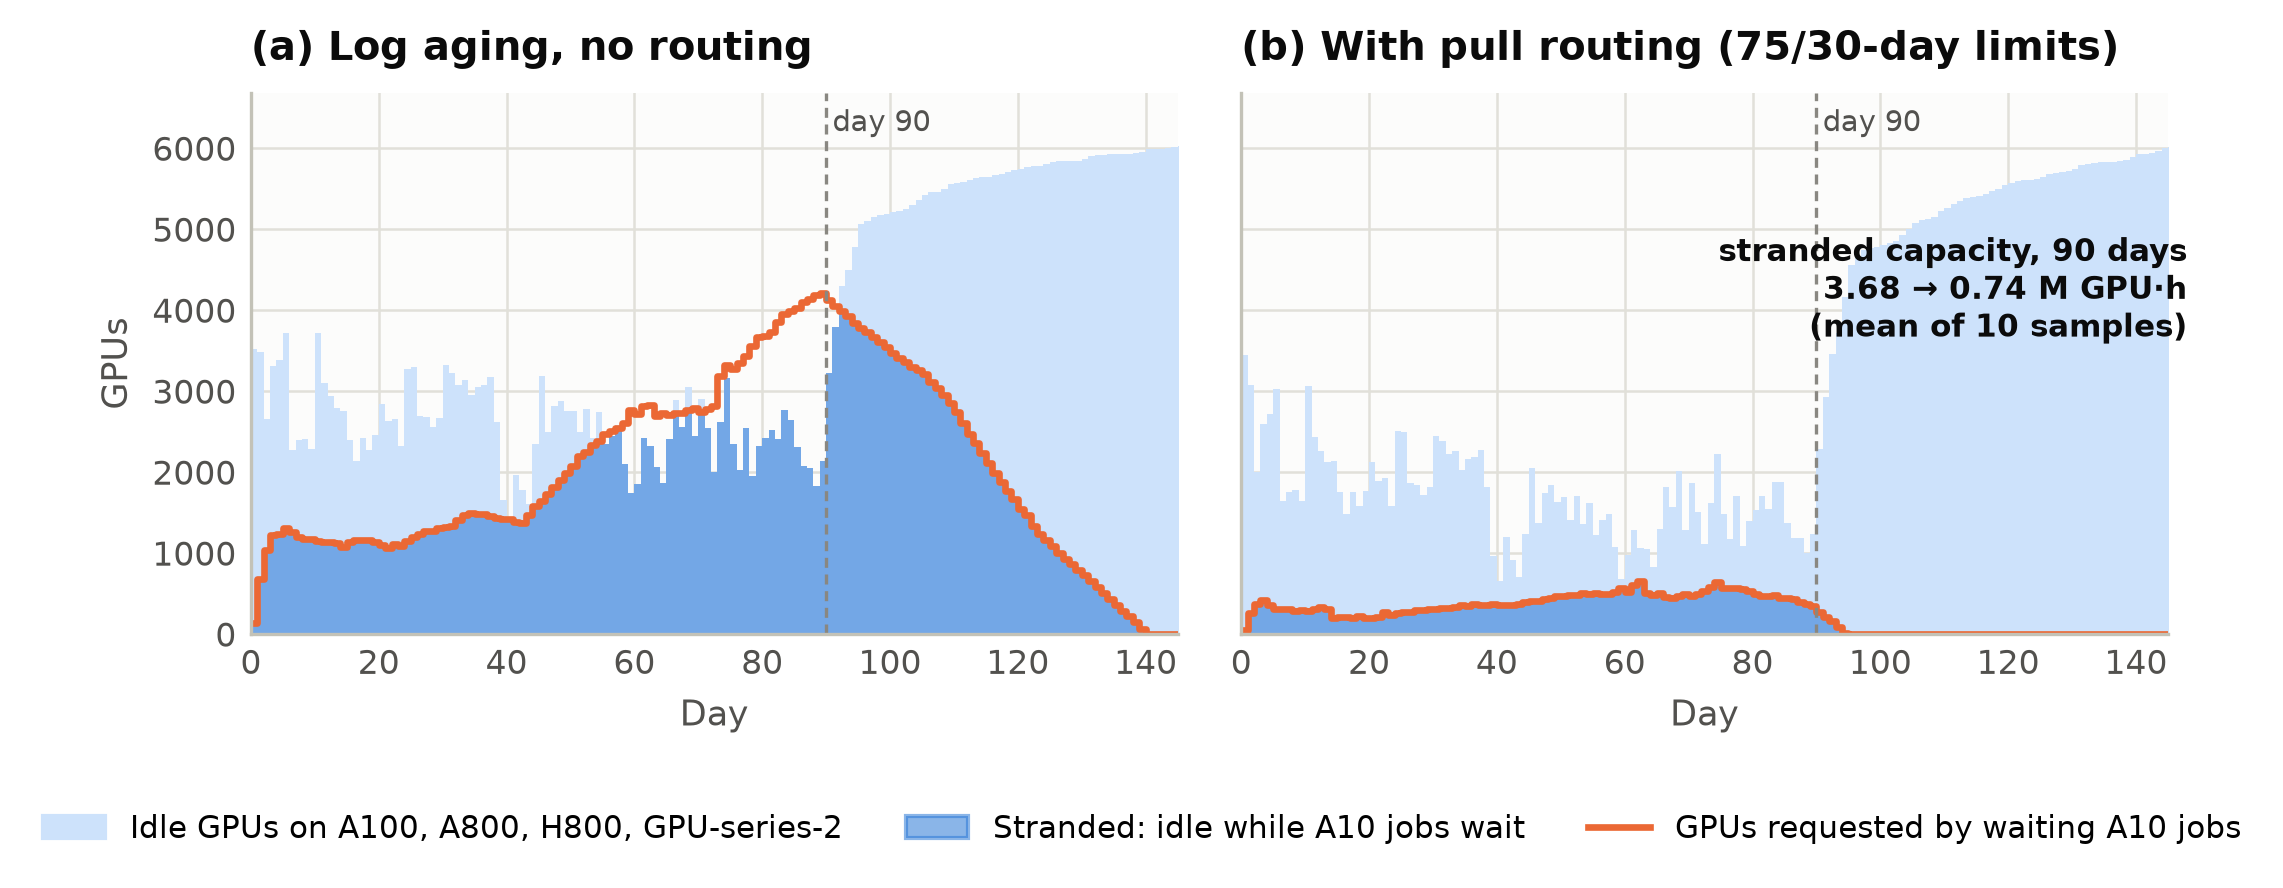
\includegraphics[width=0.97\textwidth]{fig4_stranded_capacity.png}
\caption{Idle donor GPUs (light), waiting A10 demand (orange) and stranded capacity (dark), daily averages for one eligibility sample: (a) without routing, (b) with the final routing rule.}\label{fig:stranded}
\end{figure}

We recover this capacity by letting donors pull work from the A10 queue, with rules that follow from the protection requirement A6. A donor takes A10 work only when its own queue is empty, so native jobs always come first. It scans the oldest eligible A10 jobs (at most 256) and starts each one that fits on its free nodes, while borrowed jobs may hold at most 25\% of its GPUs and vCPUs. Routed jobs run to completion on the donor, and pools are offered work in a fixed order, A100 before H800.

Two of these choices deserve explanation. We let donors \emph{pull} work rather than deciding a job's model once at submission, because capacity on a donor often frees up long after an A10 job has arrived. A one-time decision would leave such a job stuck in the A10 queue, whereas pulling revisits the waiting jobs every time a donor has room, oldest first. We offer work to A100 first because it has the most idle GPUs and narrow native jobs. In a development test with the order reversed, the mean wait of native H800 jobs rose by about 130\,h, a direct consequence of the wide H800 jobs described in Section~2.

These rules protect donors only at the moment of borrowing. The remaining harm arrives later, when a borrowed job that runs for weeks keeps its GPUs busy and native arrivals find the pool partly occupied. We therefore add a runtime limit: job $j$ may run on pool $m$ only if $d_j/v\le D_m$, and no job longer than 75 days is eligible at all. Choosing $D_m$ is the central design decision.

\subsection{Choosing the runtime limit}

We tuned the limit on three development samples of eligible jobs and froze the rule before validating it on new samples. Table~\ref{tab:limit} and Figure~\ref{fig:limit} show the trade-off for a common limit $D$ at $v=1$. Allowing longer jobs to move steadily lowers the cluster mean wait. Up to 45 days the donors bear no cost; cost appears only once loans last for months, and at 90 days the donors' 95th-percentile wait crosses the 2\,h limit. We take $D=75$ days, the largest limit that satisfies A6 on every development sample. Alternatives fare worse: an extra one-hour wait before routing raises the mean wait at every limit, a 10\% borrowing cap without a runtime limit reaches only 12.1\,h, and a 15\% cap already violates A6.

\begin{table}[ht]
\centering\small
\caption{Effect of a common runtime limit on development samples ($v=1$).}\label{tab:limit}
\begin{tabular}{lrrrrrr}
\toprule
Runtime limit $D$ & 30 d & 45 d & 60 d & 75 d & 90 d & none\\
\midrule
Cluster mean wait (h) & 15.8 & 10.8 & 6.8 & 3.6 & 2.3 & 1.4\\
Worst donor $\Delta$mean (h) & 0.00 & 0.00 & 0.05 & 0.29 & 0.45 & 1.14\\
Worst donor $\Delta$P95 (h) & 0.0 & 0.0 & 0.0 & 1.0 & \textbf{2.1} & \textbf{6.9}\\
\bottomrule
\end{tabular}
\end{table}

\begin{figure}[ht]
\centering
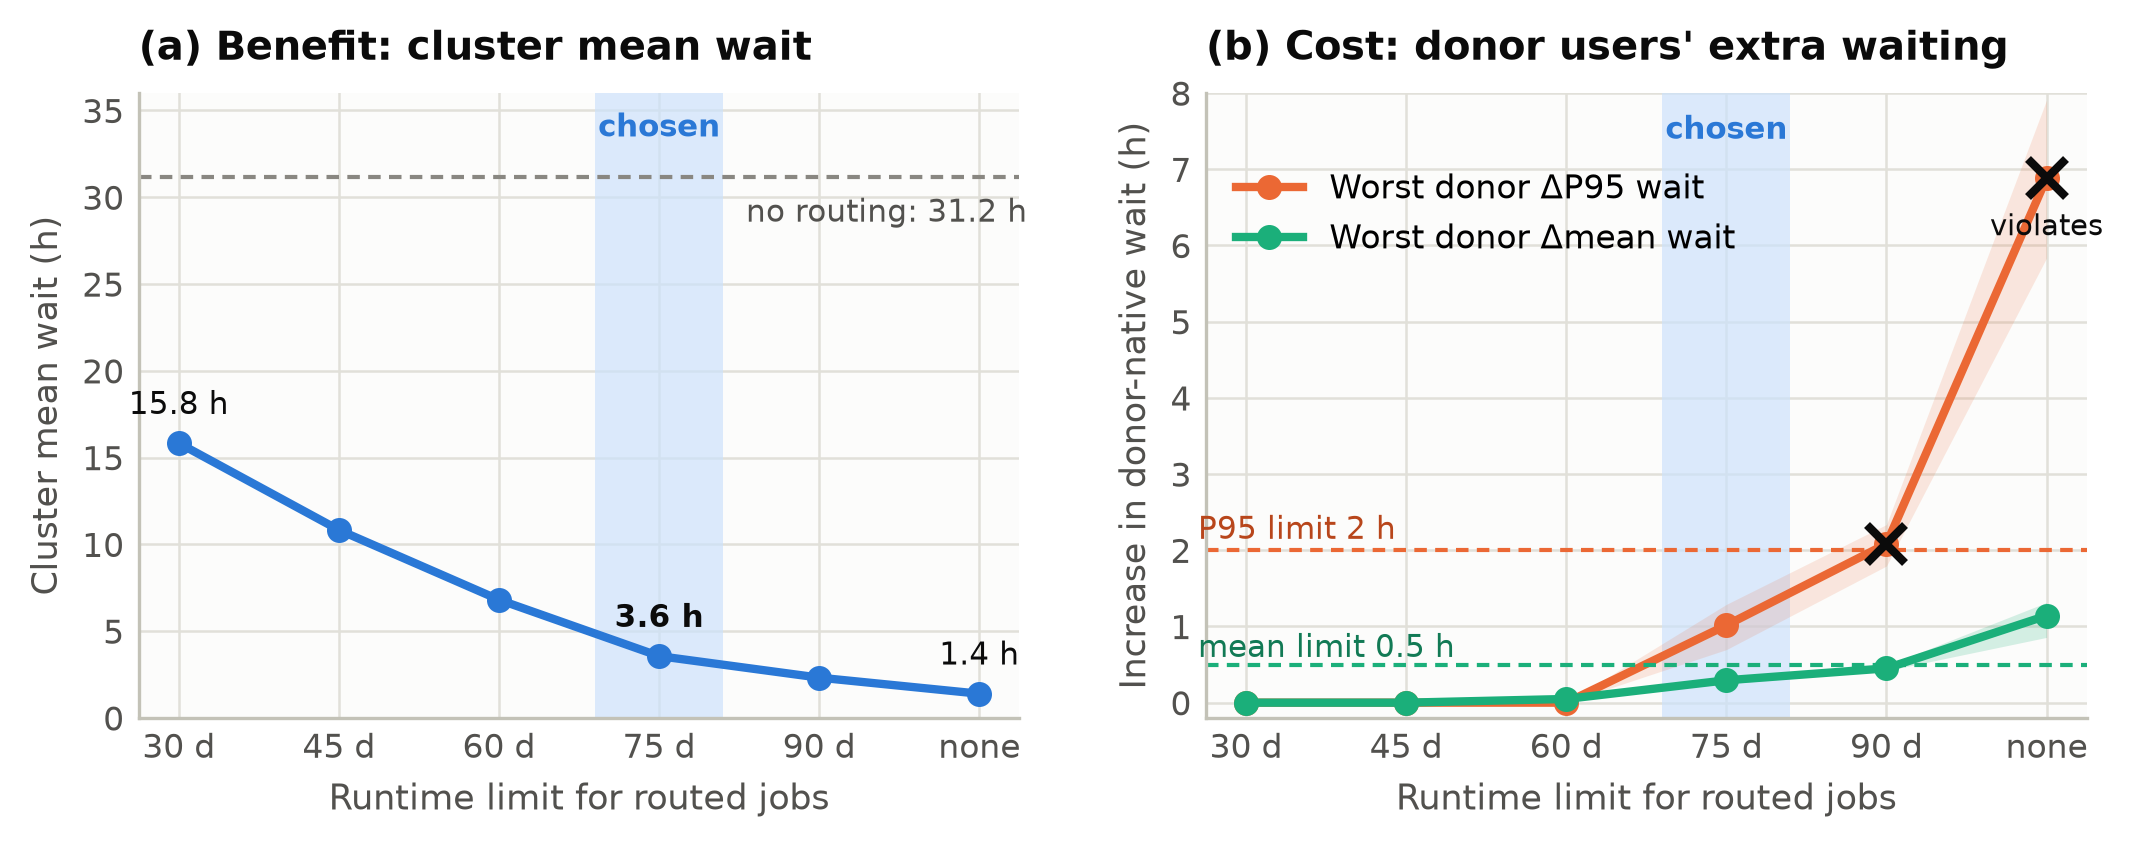
\includegraphics[width=0.97\textwidth]{fig5_runtime_limit.png}
\caption{Development samples (mean and range over three seeds): (a) cluster mean wait and (b) worst increases in donor-native waiting as the runtime limit grows. Crosses mark violations of A6.}\label{fig:limit}
\end{figure}

A common limit, however, hides the difference between donors noted in Section~2. With slower migrated jobs ($v=0.8$), borrowed jobs stay 25\% longer and H800's native 95th-percentile wait rose by 4.8\,h, violating A6. H800 is vulnerable because its native jobs are wide: a job that needs many GPUs at once must wait until enough are free together, and long-lived borrowed jobs make such moments rarer. We therefore keep $D_{\text{A100}}=75$ days and set $D_{\text{H800}}=30$ days. On the development samples this rule satisfies A6 at both speeds, with worst donor increases of 0.21\,h in the mean and 0.51\,h at the 95th percentile when $v=0.8$, and it costs only 0.5\% in mean wait at $v=1$.

\subsection{Validation}

A rule tuned on three samples could fit the particular eligible jobs in those samples rather than the workload as a whole. We therefore froze the limits and validated the rule on ten new samples of eligible jobs at each speed (Table~\ref{tab:final}); none of these samples influenced any design choice. At equal speed, routing moves 20.6\% of A10 work to the donors and recovers 80\% of the stranded capacity (Figure~\ref{fig:stranded}b). It lowers the cluster mean wait by 88\%, from 31.2\,h to 3.6\,h, and the maximum wait by 57\%. The last job finishes on day 211, 36 days earlier than without routing. Donor users pay at most 0.22\,h of additional mean wait. With 20\% slower migration, the mean wait rises to 6.8\,h, but the rule still meets A6 in all ten samples, which is what the pool-specific limits were designed to achieve.

\begin{table}[ht]
\centering\small
\caption{Final comparison: means over ten held-out samples, worst case in brackets. \emph{Routing} is the rule of Section~4.2; \emph{Protected} adds the mechanism of Section~4.4.}\label{tab:final}
\setlength{\tabcolsep}{4pt}
\begin{tabular}{lrrrrr}
\toprule
 & No & \multicolumn{2}{c}{Routing} & \multicolumn{2}{c}{Protected}\\
\cmidrule(lr){3-4}\cmidrule(lr){5-6}
 & routing & $v{=}1$ & $v{=}0.8$ & $v{=}1$ & $v{=}0.8$\\
\midrule
Cluster mean wait (h) & 31.2 & \textbf{3.60} & 6.83 & 10.50 & 14.84\\
A10 mean wait (h) & 62.4 & 6.7 & 13.2 & 20.5 & 29.3\\
Max wait (h) & 1,515 & 650 [662] & 789 [813] & 1,515 & 1,515\\
Last completion (d) & 247.1 & \textbf{211.1} & 216.8 & 247.1 & 247.1\\
Stranded capacity (M GPUh) & 3.68 & 0.74 & 1.32 & 1.43 & 1.92\\
Donor $\Delta$mean (h) & -- & 0.20 [0.22] & 0.19 [0.29] & 0.20 [0.23] & 0.18 [0.29]\\
Donor $\Delta$P95 (h) & -- & 0.39 [0.51] & 0.48 [1.04] & 0.40 [0.59] & 0.51 [1.27]\\
Samples meeting A6 & -- & 10/10 & 10/10 & 10/10 & 10/10\\
A10 jobs starting later & -- & 28.3\% & 28.8\% & \textbf{0\%} & \textbf{0\%}\\
\bottomrule
\end{tabular}
\end{table}

\subsection{Fairness inside the A10 pool}

The averages hide one more effect. Routing cuts the A10 mean wait from 62.4\,h to 6.7\,h, yet 28.3\% of A10 jobs start later than they would without routing. These delays are small, 0.28\,h per delayed job on average and 8,800 job-hours in total against 6.2 million saved. They fall mostly on jobs shorter than one day and arise because routing changes the order in which A10 resources are released.

For an operator who cannot accept any such delay, we add a protected mode. The scheduler runs, online, a shadow copy of the A10 pool under \Qstar\ without routing. Whenever the shadow starts a job that is still waiting in reality, the real scheduler starts it at the same moment on the same nodes, so no job starts later than without routing. When a shadow job holds nodes that its real counterpart no longer needs, because that job migrated or started early, the reservation becomes a loan. A waiting job may use a loaned node only if it finishes before the reservation expires. The mechanism uses only arrived jobs and known runtimes. In all twenty validation cases no A10 job starts later than under \Qstar\ (Figure~\ref{fig:valid}c). The guarantee costs efficiency: the mean wait triples from 3.6\,h to 10.5\,h and the last completion returns to day 247, mostly because the A10 jobs longer than 75 days, which cannot migrate, keep their original start times.

\begin{figure}[ht]
\centering
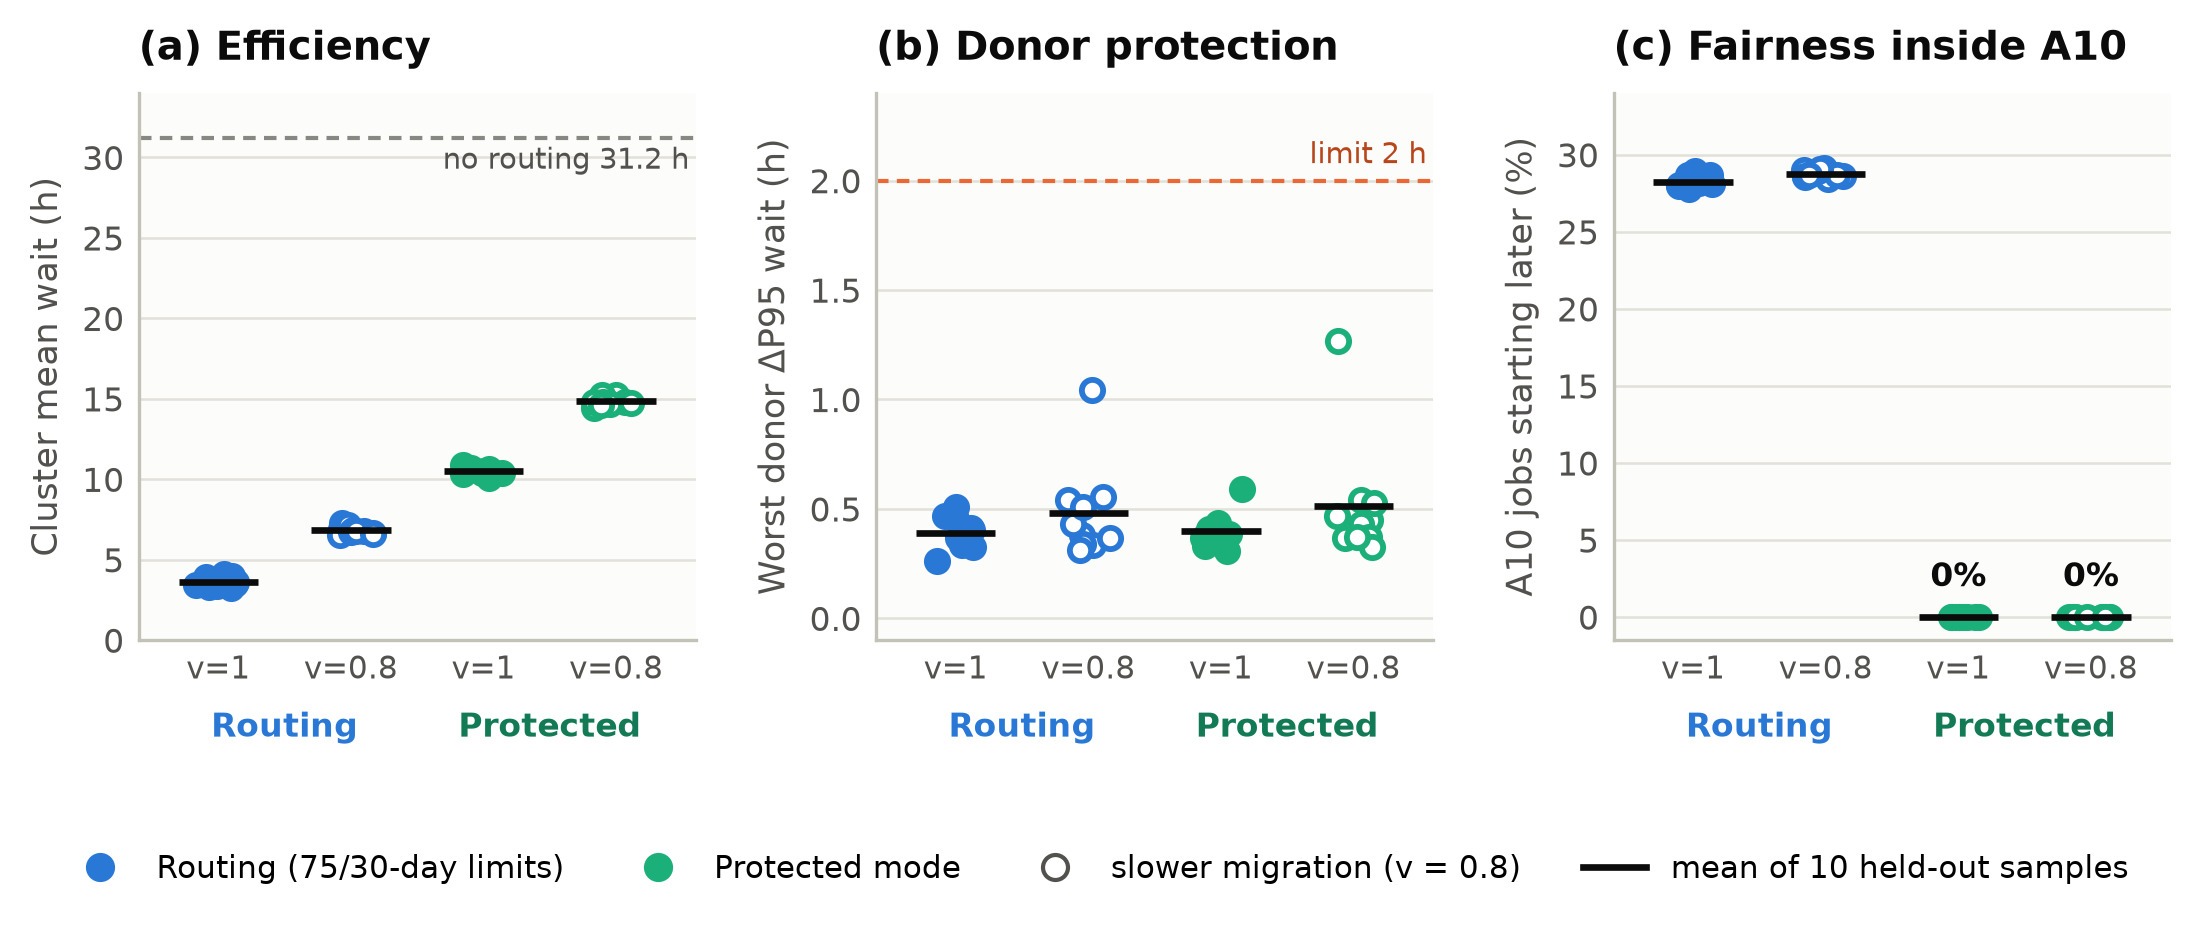
\includegraphics[width=0.97\textwidth]{fig6_validation.png}
\caption{Ten held-out samples per configuration: (a) cluster mean wait, (b) worst donor P95 increase against the 2\,h limit, (c) share of A10 jobs starting later than without routing. Hollow markers: migration at 80\% speed.}\label{fig:valid}
\end{figure}

\subsection{Sensitivity of the conclusions}

Each part of the design has been tested against the parameter it depends on most, and the conclusions respond in predictable ways. The aging constant $T$ moves the queue policy along a smooth trade-off curve: $T=30$ days favors the mean, and $T=7$ days favors the worst case. Neither choice affects the routing results qualitatively, because routing acts on the A10 backlog that every queue policy leaves behind. The runtime limit $D$ trades A10 relief against donor cost monotonically (Table~\ref{tab:limit}), and the pool-specific limits keep that cost within bounds when migrated jobs run 20\% slower. Across the ten held-out samples, the cluster mean wait under routing varies only between 3.2\,h and 4.1\,h, so the result does not hinge on which particular A10 jobs are eligible. The participation share $p$ is the one parameter that must be capped rather than maximized: with a 60-day limit, raising $p$ to 1 pushed the donors' 95th-percentile cost beyond the 2\,h limit. This observation links the scheduling design to the economic side of the problem.

\subsection{Participation and compensation}

The technical mechanism needs an economic counterpart, because the share $p$ of A10 jobs that accept substitution is set by users. A natural instrument is a discount for jobs that agree to run on another model, offered to a limited quota rather than to everyone: raising $p$ from 0.5 to 1 pushed the donors' 95th-percentile cost above 5\,h. The delays that remain for donor users can be compensated by a delay credit equal to each delayed native job's extra wait times its GPU count. Under our rule, total credits come to 3.1\% of the GPU-weighted waiting saved by A10 jobs; measured in plain job-hours, A10 jobs save 392 hours for every hour added to donor users. A small fraction of the gain therefore makes donor users whole. The credits could be redeemed as a price discount or as a one-time priority boost on a later job, and because they are computed from the scheduler's own logs, the account is fully auditable. A more aggressive scheme without runtime limits, relying on compensation alone, reached a 1.4\,h mean wait but met its own acceptance criteria in only 3 of 10 held-out samples, and we do not recommend it.

\section{Strengths and Weaknesses}

Our approach takes the constraints literally. Placement is checked node by node with simultaneous worker starts and fractional CPUs, and every job runs to completion, so no result depends on truncating the trace. Every parameter was chosen on development samples and confirmed on unused ones, every saved schedule passes an independent exact-arithmetic audit, and 187 unit tests check the rules' mathematical properties. The recommended system has few controls, each with a direct operational meaning: the aging constant $T$, the runtime limits $D_m$ and the participation share $p$.

The main weakness is that all of this rests on a single trace: validation varies which jobs may migrate, not the workload, and another month of submissions could favor different parameters. Runtimes are treated as exact, migration overhead, memory and topology are ignored, and cross-model compatibility and speed are assumptions. Strict head blocking wastes some capacity in pools with wide jobs, so combining logarithmic aging with backfilling is a natural next step. We also leave the mildly overloaded GPU-series-1 pool unaddressed; partitioning high-end GPUs into smaller instances (NVIDIA MIG) could add capacity for A10-sized jobs.

\section{Conclusions and Recommendations}

The three questions of this problem form a single chain. The data analysis showed that the cluster's difficulty has two separate sources: work concentrated in a few long jobs, and an A10 pool with about half the capacity its users need. The first is a matter of order, which a queue policy can address. Logarithmic aging serves short jobs almost as quickly as shortest-job-first while keeping the worst wait near the first-come-first-served level. The second is a matter of capacity, which no queue policy can address. Pull routing with pool-specific runtime limits moves a fifth of the A10 work onto idle A100 and H800 GPUs, cutting the cluster mean wait from 31.2\,h to 3.6\,h at a negligible cost to the donor pools.

Figure~\ref{fig:tails} summarizes the progression in a single picture: the share of jobs that wait longer than a given time, for each schedule we built. FCFS keeps about half of all jobs waiting for hundreds of hours. SJF and \Qstar\ remove almost all of that waiting but differ in the extreme tail, where \Qstar\ cuts off near the FCFS maximum while SJF reaches 3,000\,h. Routing then lowers the curve at almost every waiting time and truncates the tail at about 700\,h. The protected variant follows the routing curve for short and moderate waits but keeps the \Qstar\ tail, because the longest A10 jobs retain their original start times.

\begin{figure}[ht]
\centering
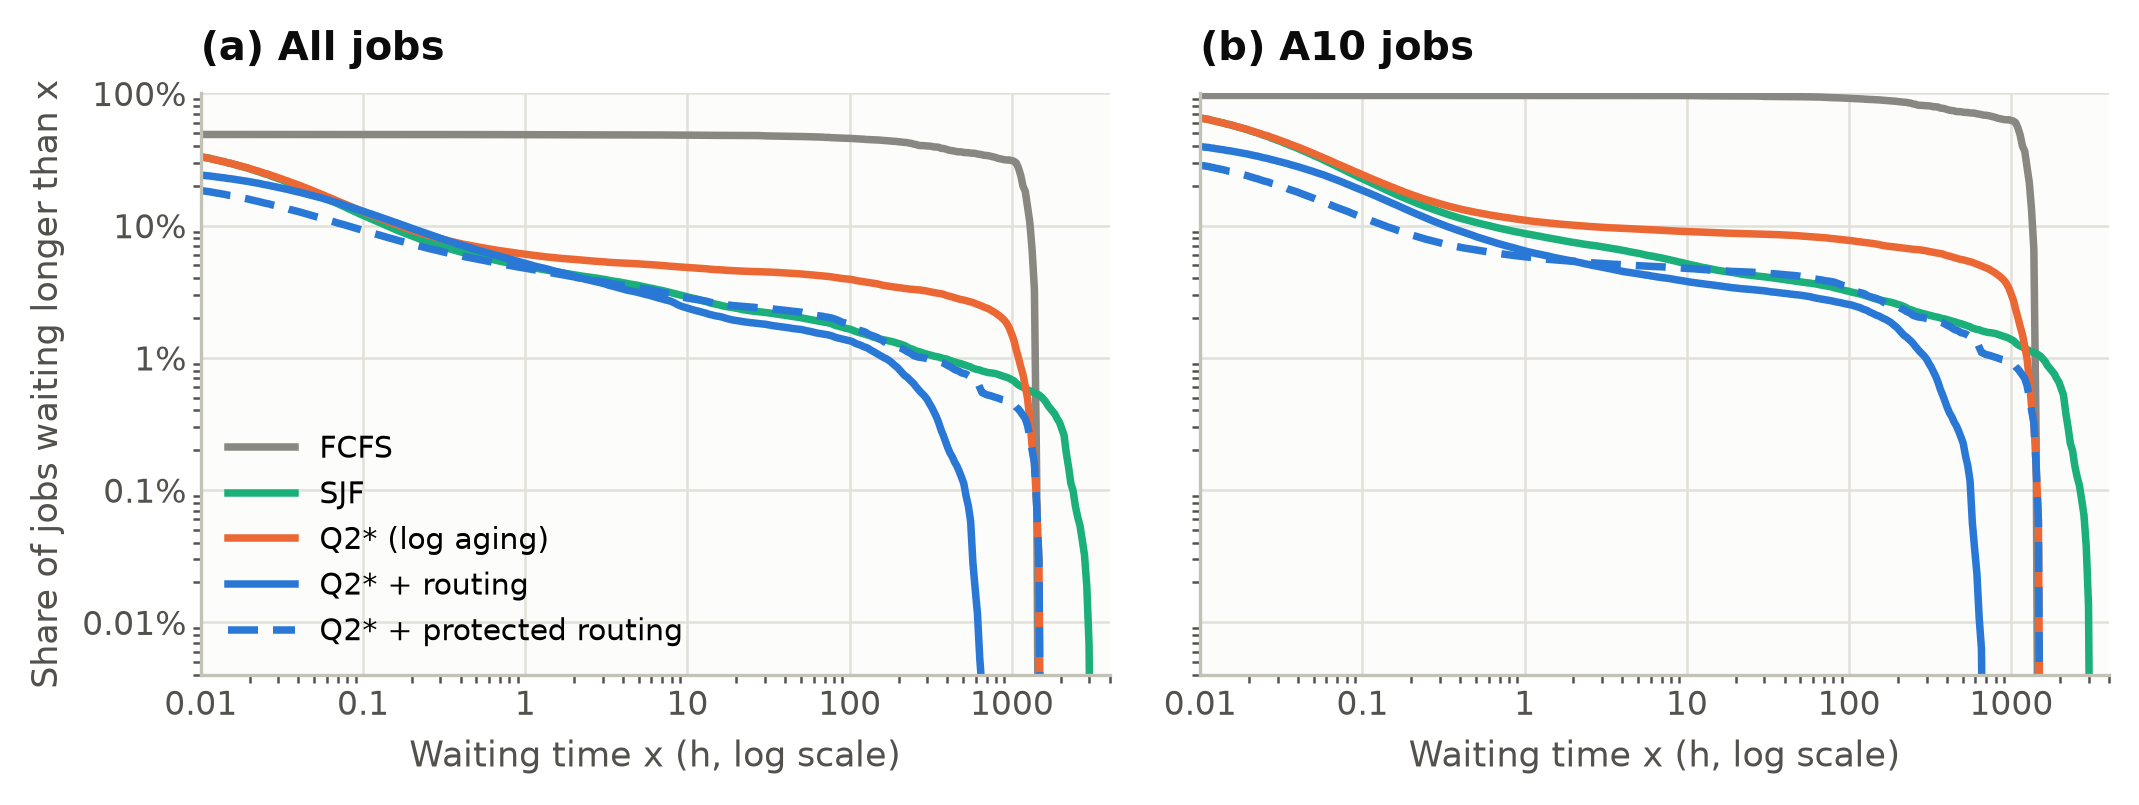
\includegraphics[width=0.97\textwidth]{fig_wait_tails.png}
\caption{Share of jobs waiting longer than $x$ hours under each schedule, (a) for all jobs and (b) for A10 jobs. Routing curves use the first held-out eligibility sample.}\label{fig:tails}
\end{figure}

These results translate into the following recommendations. Within every pool, the cluster should order its queues by logarithmic aging with $T=7$ days, which keeps short jobs responsive while preventing the months-long starvation of SJF; $T$ can be raised if average responsiveness matters more than the worst case. Across pools, it should invite about half of A10 jobs to accept substitution and let idle A100 and then H800 GPUs pull them, with each donor lending at most 25\% of its capacity and accepting jobs of at most 75 days (A100) or 30 days (H800). The operator should monitor each donor's native mean and 95th-percentile wait, the share of A10 jobs that start later, and the delay-credit ratio, and should switch to the protected mode if A10 users must be guaranteed that routing never delays them. Together, these measures lower the cluster mean wait from 447\,h under FCFS to under 4\,h and finish the trace 32 days earlier, while the donor pools keep an explicit service guarantee.

\begin{thebibliography}{5}\small
\setlength{\itemsep}{0pt}
\bibitem{prob} 2026 MCM Senior Group Problem B, \emph{Scheduling a GPU Cluster}, with \texttt{node\_info\_df.csv} and \texttt{job\_info\_clean.csv}.
\bibitem{ali} Alibaba Group. Alibaba Cluster Trace Program (GPU trace). \url{https://github.com/alibaba/clusterdata}
\bibitem{lifka} D.~Lifka. The ANL/IBM SP scheduling system. \emph{Job Scheduling Strategies for Parallel Processing}, LNCS 949, pp.~295--303, 1995.
\bibitem{slurm} SchedMD. Slurm Scheduling Configuration Guide. \url{https://slurm.schedmd.com/sched_config.html}
\bibitem{mig} NVIDIA. Multi-Instance GPU User Guide. \url{https://docs.nvidia.com/datacenter/tesla/mig-user-guide/}
\end{thebibliography}

\section*{Use of AI Tools}

We used Anthropic Claude to compare the candidate problems, review intermediate results, write experiment specifications, and draft this report, and OpenAI Codex to implement the analysis and simulation code, run the experiments, produce verification scripts, and draft working notes. All modeling choices and conclusions were reviewed by the authors, who take full responsibility for the submission.

\end{document}
